\section{Step 3 - Boolean Operations}
\subsection{What are Boolean Operations?}
In the last step we learned how to construct spheres.
Spheres are a member some sort of objects called primitives.
Combining primitives can be used to build more complicated structures.
Think of combinations like add, subtract and difference.
For example you may ask for the volume which is occupied by a sphere without the volume occupied by another sphere.

If you've taken set theory at school you probably drawed so called Venn diagrams.
These diagrams work analog to the Boolean operations offered in {\tt pythonOCC}.
Figure~\ref{BOOLEAN_COMBINATIONS_OF_SETS} illustrates the Boolean operations of two overlapping sets $A$ and $B$ utilising Venn diagrams.
% +++++++++++++++++++++++++++++++++++++++++++++++++++++++++++++++++++++++ 
\begin{figure}[htbp]
  \centering
  \subfigure[Set A]{
    \label{SET_A}
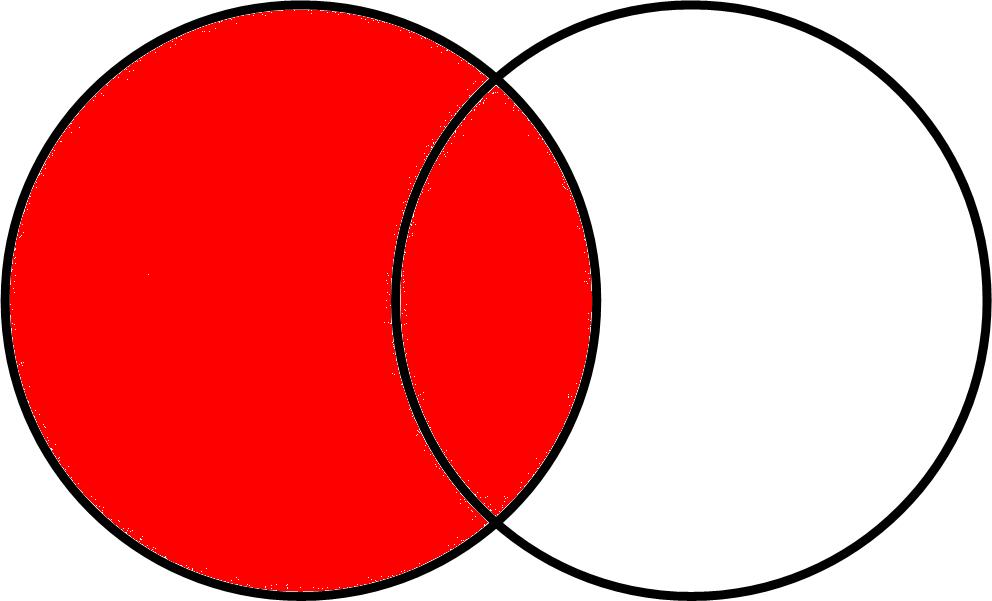
\includegraphics[height=2.862cm,width=4.725cm]{SetA.jpg}
  }
  \hspace{0.5cm} % Abstand zwischen den subfigures
  \subfigure[Set B]{
    \label{SET_B}
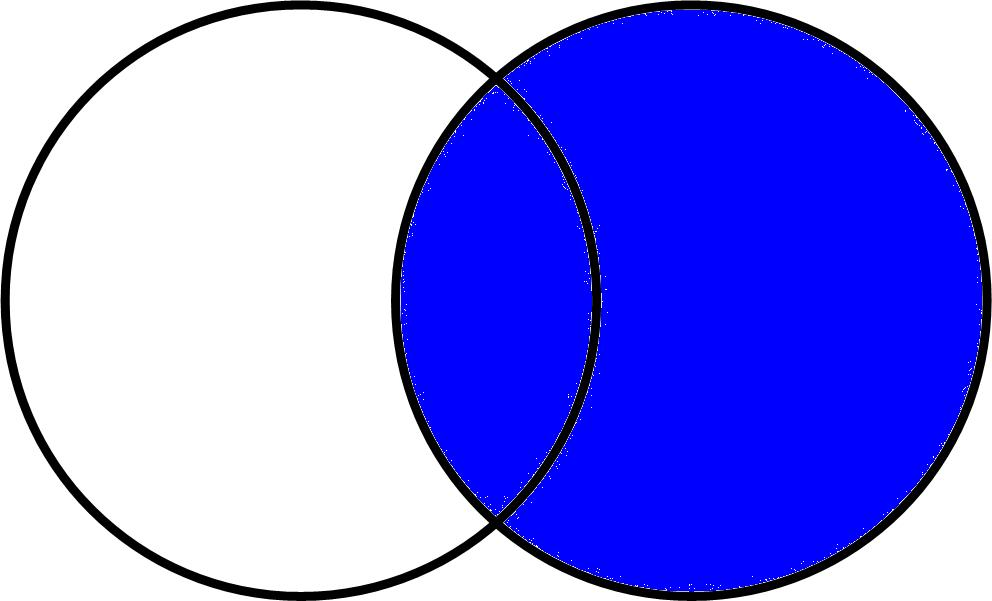
\includegraphics[height=2.862cm,width=4.725cm]{SetB.jpg}
	}  
  \hspace{0.5cm} % Abstand zwischen den subfigures
  \subfigure[Set A or set B $\;(A \cup B)$]{
    \label{SET_A_OR_SET_B}
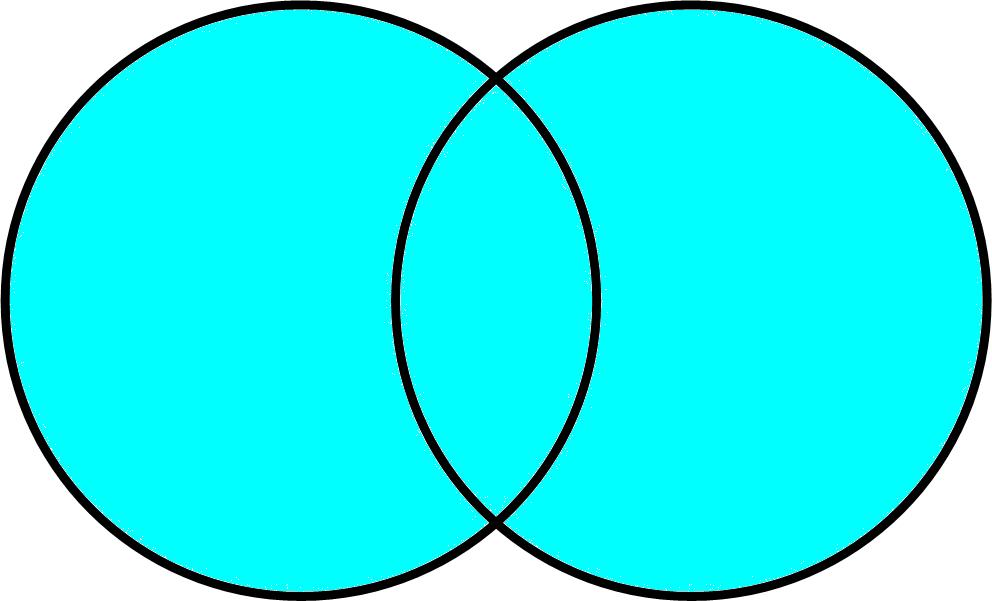
\includegraphics[height=2.862cm,width=4.725cm]{SetAOrB.jpg}
	}  

  \vspace{0.3cm} % Abstand zwischen den subfigures
  \subfigure[Set A and set B $\;(A \cap B)$]{
    \label{SET_A_AND_SET_B}
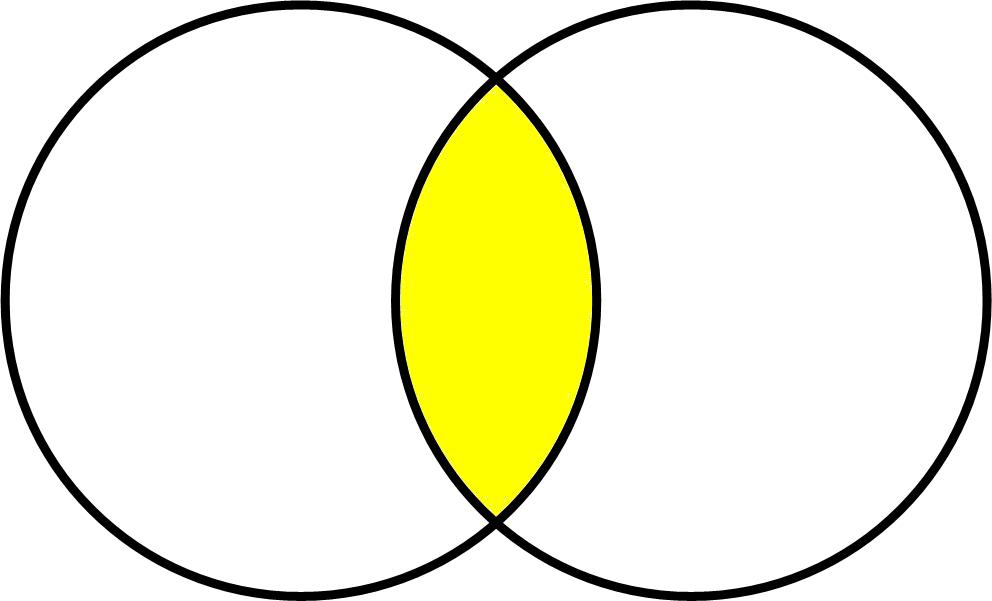
\includegraphics[height=2.862cm,width=4.725cm]{SetAAndB.jpg}
  }
  \hspace{0.5cm} % Abstand zwischen den subfigures
  \subfigure[Set A without set B $\;(A \setminus B)$]{
    \label{SET_A_WITHOUT_SET_B}
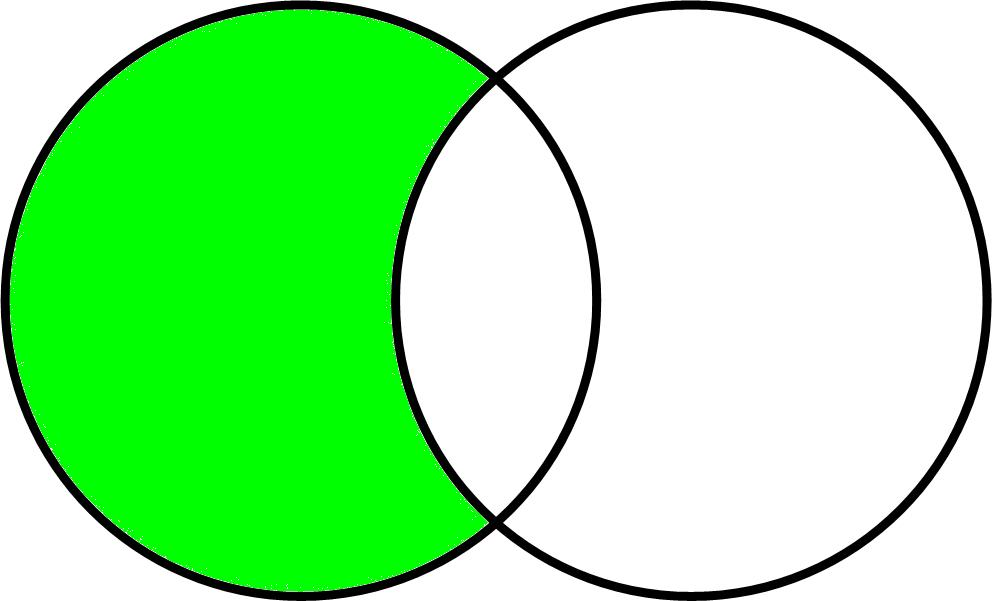
\includegraphics[height=2.862cm,width=4.725cm]{SetAOhneB.jpg}
	}  
  \hspace{0.5cm} % Abstand zwischen den subfigures
  \subfigure[Set B without set A $\;(B \setminus A)$]{
    \label{SET_B_WITHOUT_SET_A}
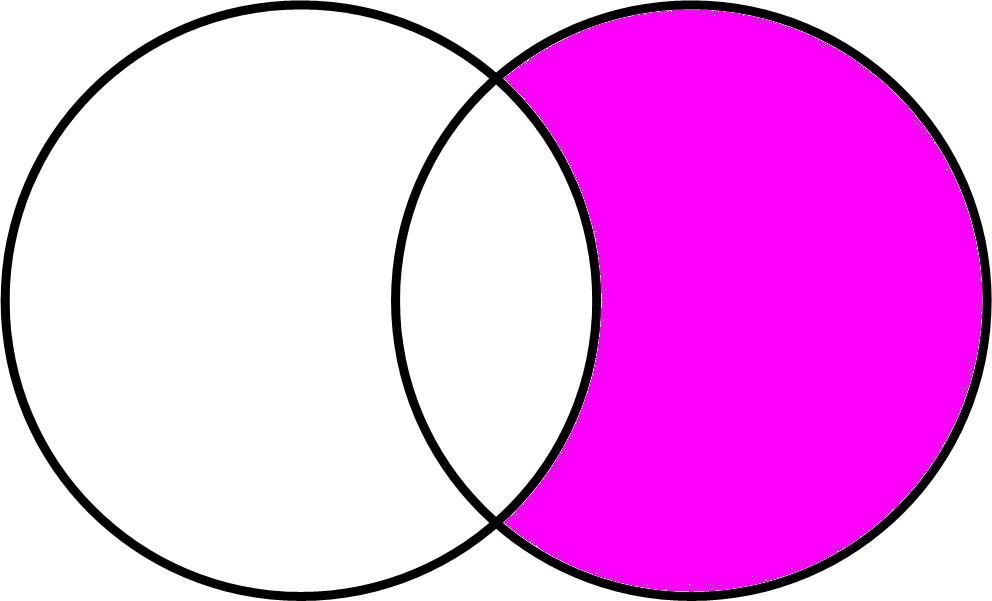
\includegraphics[height=2.862cm,width=4.725cm]{SetBOhneA.jpg}
	}  
 \vspace{0.3cm}
  \caption[Sets and their Boolean combinations]{Sets and their Boolean combinations}
  \label{BOOLEAN_COMBINATIONS_OF_SETS}
\end{figure}

If you created two primitives {\tt pythonOCC} can perform Boolean operations analog to those sketched in figure~\ref{BOOLEAN_COMBINATIONS_OF_SETS}.
Sometimes this is called {\it Constructive Solid Geometry (CSG)}.
You need to import {\tt OCC.BRepAlgoAPI} into your code because this functionality resides in that module.
The main functions are:
\begin{enumerate}
\item {\tt BRepAlgoAPI\_Fuse} combines two primitives so that the 
		resulting object occupies the space of both source objects. 
		This is equivalent to the {\tt or}-operation (symbol $\cup$) shown in
		figure~\ref{SET_A_OR_SET_B}.
\item {\tt BRepAlgoAPI\_Common} combines two primitives so that the 
		resulting object occupies the overlapping space of both source objects. 
		This is equivalent to the {\tt and}-operation (symbol $\cap$) shown in
		figure~\ref{SET_A_AND_SET_B}.
\item {\tt BRepAlgoAPI\_Cut} combines two primitives so that the 
		resulting object occupies the space of the first source object minus the 
		space ocuppied by the second source object. 
		This is equivalent to the {\tt without}-operation (symbol $\setminus$)
		shown in figures~\ref{SET_A_WITHOUT_SET_B} and~\ref{SET_B_WITHOUT_SET_A}.
\end{enumerate}

\subsection{A first sample on Boolean operations in pythonOCC}
In order to see how things work execute sample {\tt Step3\_1.py}, click on menu {\tt Draw} menu-item  {\tt draw sphere 1} and after that click on menu {\tt Draw} menu-item  {\tt draw sphere 2}.
Please note that before drawing the new object the screen is erased.
Use the new menu  {\tt Boolean} and select the menu-items.
Turn the objects so you can see their shape.

The menu-items should be self explaining so let's look at the code.
Listing~\ref{LISTING_STEP3_1_PY_A} shows how the menu and menu-items were changed to make the new funcionality available in the graphical use interface.
\begin{python}[moreemph={[4], 46, 48},caption={Step3\_1.py - Extending the menu},label=LISTING_STEP3_1_PY_A]
...
    # This is the place where we hook our functionality to menus
    # ----------------------------------------------------------
    add_menu('File')
    add_function_to_menu('File',  exit)
    add_menu('Draw')
    add_function_to_menu('Draw', draw_sphere_1)
    add_function_to_menu('Draw', draw_sphere_2)
    add_menu('Boolean')
    add_function_to_menu('Boolean', draw_fused_spheres)
    add_function_to_menu('Boolean', draw_cutted_spheres_1)
    add_function_to_menu('Boolean', draw_cutted_spheres_2)
    add_function_to_menu('Boolean', draw_common_spheres)
    add_menu('Erase')
    add_function_to_menu('Erase', erase_all)
...    
\end{python}
This should not be a suprise if you studied the code of the former steps.
So in the next step we do not discuss that anymore.
If you are unsure look at the code.

Listing~\ref{LISTING_STEP3_1_PY_B} shows two of the new functions added under menu {\tt Boolean}.
%
\begin{python}[moreemph={[4], 46, 48},caption={Step3\_1.py - Extending the functionality},label=LISTING_STEP3_1_PY_B]
def draw_cutted_spheres_2(event=None):
    # clear the display
    display.EraseAll()
    # create sphere
    Radius = 50.0
    # The sphere center as a Scipy array - 3 rows, one column
    # Note we use the scipy.zeros function
    PointZeroArray = scipy.zeros((3,1), dtype=float)
    MySphere1 = sphere_from_vector_and_radius(  PointZeroArray, 
                                                Radius )
    MySphere1Shape = MySphere1.Shape()

    # The sphere center as a Scipy array - 3 rows, one column
    MyPointAsArray = scipy.array([25.0, 50.0, 50.0])
    MyPointAsArray = scipy.reshape(MyPointAsArray,(3,1))
    MySphere2 = sphere_from_vector_and_radius(  MyPointAsArray, 
                                                Radius )
    MySphere2Shape = MySphere2.Shape()
    # Combine the spheres
    CuttedSpheres = OCC.BRepAlgoAPI.BRepAlgoAPI_Cut(    MySphere2Shape, 
                                                        MySphere1Shape )
    # Shape of combined spheres
    CuttedSpheres = CuttedSpheres.Shape()
    # Display 
    display.DisplayColoredShape( CuttedSpheres , 'BLUE' ) 

def draw_common_spheres(event=None):
    # clear the display
    display.EraseAll()
    # create sphere
    Radius = 50.0
    # The sphere center as a Scipy array - 3 rows, one column
    # Note we use the scipy.zeros function
    PointZeroArray = scipy.zeros((3,1), dtype=float)
    MySphere1 = sphere_from_vector_and_radius(  PointZeroArray, 
                                                Radius )
    MySphere1Shape = MySphere1.Shape()

    # The sphere center as a Scipy array - 3 rows, one column
    MyPointAsArray = scipy.array([25.0, 50.0, 50.0])
    MyPointAsArray = scipy.reshape(MyPointAsArray,(3,1))
    MySphere2 = sphere_from_vector_and_radius(  MyPointAsArray, 
                                                Radius )
    MySphere2Shape = MySphere2.Shape()
    # Combine the spheres
    CommonSpheres = OCC.BRepAlgoAPI.BRepAlgoAPI_Common( MySphere1Shape, 
                                                        MySphere2Shape )
    # Shape of combined spheres
    CommonSpheres = CommonSpheres.Shape()
    # Display 
    display.DisplayColoredShape( CommonSpheres , 'GREEN' ) 
...    
\end{python}
At the beginning of these functions the canvas is erased.
After that two sphere shapes are created in exactly the same manner as in listing \ref{LISTING_STEP2_2_PY_A}.
The next lines provide something new.
As the comment tells the spheres are combined.

Function {\tt draw\_cutted\_spheres\_2} performs the Boolean {\it without} operation utilising the function {\tt BRepAlgoAPI\_Cut}.
The function takes two shapes of primitives and delivers the result first primitive without second primitive.
If you change the order of the arguments given to function {\tt BRepAlgoAPI\_Cut} the Boolean operation is also changed like shown in function {\tt draw\_cutted\_spheres\_1}.

Next we look at function {\tt draw\_common\_spheres}.
Note that the function is similar to function {\tt draw\_cutted\_spheres\_2}.
The Boolean operation is the main difference between these functions.
In {\tt draw\_common\_spheres} function {\tt BRepAlgoAPI\_Common} is used to perform the {\tt and} operation.

Please note the similarity of both Boolean operations discussed.
Combing two primitives is always done in the same manner.
\begin{enumerate}
\item Construct {\tt Primitive\_1}
\item Create the shape {\tt Shape\_1 = Primitive\_1.Shape()}
\item Construct {\tt Primitive\_2}
\item Create the shape {\tt Shape\_2 = Primitive\_2.Shape()}
\item Perform the Boolean operation between {\tt Shape\_1} and  {\tt Shape\_2} to get a {\tt New\_Object}
\item Create {\tt New\_Object.Shape()} before displaying it
\end{enumerate}

\subsection{Extending the first sample on Boolean operations in pythonOCC}
\subsubsection{What we want to do and how it looks like}
Now that we know how to construct and combine primitives we should practice our new abilities.
What about drawing other things like a cylinder, a cone and an arrow?
Oh no, unfortunately there is no primitive creating arrows available.
So forget about the last one.
Stop!
We learned how to use Boolean operations so lets use a cone and a cylinder for the arrow and combine these.

Execute {\tt Step3\_2.py} to see how we extend our sample.
Please use menu {\tt Draw} and try the new functions {\tt draw cylinder},  {\tt draw cone} and  {\tt draw arrow}.
Also note that in contrast to {\tt Step3\_1.py} the functions under menu {\tt Draw} do not erase the canvas.
Hence all objects remain there until you use function {\tt erase all} or until you use one of the items under menu {\tt Boolean} or until you close the program.
Figure~\ref{STEP_3_2_SCREEN} shows how the canvas can look if you choose all objects from menu {\tt Draw}.
If you do the same you will see the objects but the perspective may differ.
% +++++++++++++++++++++++++++++++++++++++++++++++++++++++++++++++++++++++ 
% +++ Bild: Step 3_2 ++++++++++++++++++++++++++++++++++++++++++++++++++++
% +++++++++++++++++++++++++++++++++++++++++++++++++++++++++++++++++++++++ 
\begin{figure}[h]
\begin{center}
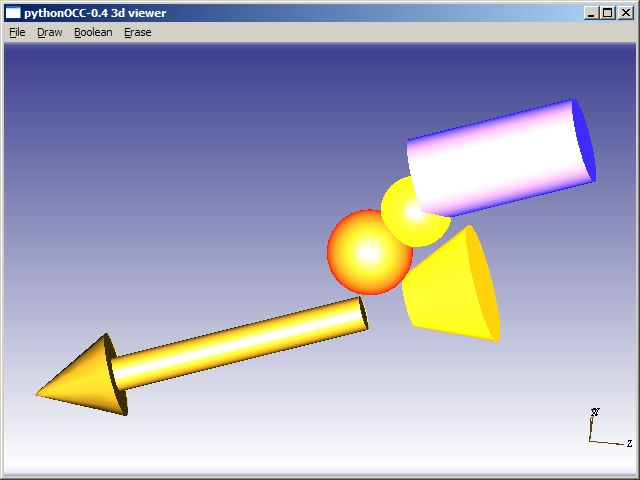
\includegraphics[height=8.5cm,width=11.3cm]{Step3_2.jpg}
\end{center}
\caption[Screenshot of Step3\_2]{\label{STEP_3_2_SCREEN}Screenshot of Step3\_2}
\end{figure}

\subsubsection{Creating a cylinder}
\label{SECT_CYLI}
We start with the creation of the cylinder object\footnote{
Maybe you ask yourself: Should I start learning how to use the OpenCascade documentation and practise beside working on that introduction?
If you want that open the  C++ documentation of Open~Cascade~\cite{OPENCASCADE_ORG} and read the constructors for a cylinder.
You don't need to do that now but you definitely have to do that if you create own applications.
So start using it whenever you think you are ready for it and learn how to go around in the docu. 
No fear! 
If you honor the structure shown in the C++ documentation and think in Python code you will learn using the application of the C++ documentation to create your own code although it is Python and not C++.
If you want to keep focused on what is presented here that's also ok. 
The intention of that hint is only to encourage the reader to use the documentation. 
To some extent the way of learning is different for every individual so you need to decide how to learn.}.
%
Listing~\ref{LISTING_STEP3_2_PY_A}\footnote{Please note the marvellous documentation strings. This is epytext a very easy markaup language for {\tt Epydoc}~\cite{EPYDOCWEB} a very efficient documentation tool. In my opinion it is worth a trial.}
presents the complete function.
Skim over it so we can go into the details in the following paragraphs.
%
\begin{python}[moreemph={[4], 46, 48},caption={Step3\_2.py - Defining a cylinder from a point, a direction vector, the length and the radius},label=LISTING_STEP3_2_PY_A]
def cylinder_from_point_directionvector_length_and_radius(  vector, 
                                                            directionvector,
                                                            length,
                                                            radius ):
    """
    Creates a cylinder utilising OCC.BRepPrimAPI.BRepPrimAPI_MakeCylinder out 
    of scipy arrays
    
    @param vector: vektor of starting point on the cylinder main axis
    @type  vector: scipy array(3,1)
    @param directionvector: direction vector of the cylinder main axis
    @type  directionvector: scipy array(3,1)
    @param length: cylinder length
    @type  length: float
    @param radius: cylinder radius
    @type  radius: float
    @return: cylinder

    sample::
    
        Vector = scipy.array([ 10.0, 10.0, 10.0 ])
        Vector = scipy.reshape( Vector, (3,1))
        
        TangUnitVector = scipy.array([  (1/scipy.sqrt(3)) , 
                                         1/scipy.sqrt(3)) , 
                                         1/scipy.sqrt(3)) ])
        TangUnitVector = scipy.reshape( TangUnitVector, (3,1))

        CylLength = 200
        CylRadius = 3
    
        Cyli = cylinder_from_point_directionvector_length_and_radius(Vector, 
                                                             TangUnitVector,
                                                             CylLength,
                                                             CylRadius ) 
        CyliShape = Cyli.Shape()
        display.DisplayColoredShape( CyliShape , 'RED' ) 
    """
    # Normalize the direction
    directionunitvector = NormVector(directionvector)
    # determine the second point
    vector2 = vector + length * directionunitvector    
    # components of vector in float values
    X1 = float( vector[ 0, 0] )
    Y1 = float( vector[ 1, 0] )
    Z1 = float( vector[ 2, 0] )
    # components of vector2 in float values
    X2 = float( vector2[ 0, 0] )
    Y2 = float( vector2[ 1, 0] )
    Z2 = float( vector2[ 2, 0] )
    # create OCC.gp.gp_Pnt-points
    P1 = OCC.gp.gp_Pnt( X1, Y1, Z1 )
    P2 = OCC.gp.gp_Pnt( X2, Y2, Z2 )
    # create direction unit vector from these points (not neccessary but if 
    # the directionunitvector is not of length 1 ...)
    directionP1P2 = scipy.array([   ( X2 - X1 ),
                                    ( Y2 - Y1 ),  
                                    ( Z2 - Z1 ) ])
    directionP1P2 = scipy.reshape( directionP1P2,(3,1))
    # distance between the points (X1, Y1, Z1) and (X2, Y2, Z2)
    length = length_column_vector(directionP1P2)
    # normalize direction
    directionP1P2 = NormVector(directionP1P2)                                                
    # origin at point 1 with OCC.gp.gp_Pnt
    origin_local_coordinate_system = OCC.gp.gp_Pnt( X1, Y1, Z1)
    # z-direction of the local coordinate system with OCC.gp.gp_Dir
    z_direction_local_coordinate_system = OCC.gp.gp_Dir(directionP1P2[0, 0], 
                                                        directionP1P2[1, 0], 
                                                        directionP1P2[2, 0])
    # local coordinate system with OCC.gp.gp_Ax2
    local_coordinate_system = OCC.gp.gp_Ax2(origin_local_coordinate_system, 
                                            z_direction_local_coordinate_system)
    # create cylinder utilising OCC.BRepPrimAPI.BRepPrimAPI_MakeCylinder
    cylinder = OCC.BRepPrimAPI.BRepPrimAPI_MakeCylinder(local_coordinate_system, 
                                                        radius, 
                                                        length, 
                                                        2 * scipy.pi )
    # return cylinder
    return cylinder
\end{python}
Function {\tt cylinder\_from\_point\_directionvector\_length\_and\_radius} is heavily commented so studying the code should be possible.
Anyhow a few words may help.
As the function name implies we construct the cylinder from a point, a direction vector, the length and the radius.
The first two parameters have to be {\tt Scipy} arrays the other two are floating point values.

We start with the normalization of the direction vector.
\begin{python}
    # Normalize the direction
    directionunitvector = NormVector(directionvector)
\end{python}
We utilize function {\tt NormVector} which uses function {\tt length\_column\_vector}.
Both functions are found in the source.
The first takes a direction vector of arbitrary length and returns a direction vector of length one with the same direction, the latter one determines the length of a vector.
\\
We get one center point at one end of the cylinder from the parameters.
So we compute the center point at the other end.
\begin{python}
    # determine the second point
    vector2 = vector + length * directionunitvector    
\end{python}
As already mentioned casting the contents of a {\tt Scipy} array to floats avoided some mysterious error messages.
Note that we do not mention that in the next sections. 
Please have a look at the following lines and try to keep them in mind.
\begin{python}
    # components of vector in float values
    X1 = float( vector[ 0, 0] )
    Y1 = float( vector[ 1, 0] )
    Z1 = float( vector[ 2, 0] )
\end{python}
The construction of points {\tt OCC.gp.gp\_Pnt} was already shown
\begin{python}
    # create OCC.gp.gp_Pnt-points
    P1 = OCC.gp.gp_Pnt( X1, Y1, Z1 )
\end{python}
but here is something new.
\begin{python}
    # z-direction of the local coordinate system with OCC.gp.gp_Dir
    z_direction_local_coordinate_system = OCC.gp.gp_Dir(directionP1P2[0, 0], 
                                                        directionP1P2[1, 0], 
                                                        directionP1P2[2, 0])
\end{python}
Thats the direction of the cylinder in {\tt pythonOCC} termonology.
It serves as a local $z$-coordinate for our cylinder primitive.
The constructor used a few lines later constructs a cylinder accoding to a local coordinate system.
The main axis of the cylinder created is the $z$-coordinate of that local coordinate system.
So it is no suprise that with
\begin{python}
    # local coordinate system with OCC.gp.gp_Ax2
    local_coordinate_system = OCC.gp.gp_Ax2(origin_local_coordinate_system, 
                                            z_direction_local_coordinate_system)
\end{python}
a local coordinate is introduced.
What about the $x$- and $y$-direction of the local coordinate system?
The answer is: I don't know.
But remember the cylinder is oriented along the $z$-axis and we do not care about $x$ and $y$.
The cross section of the cylinder is a circle so who cares about that?
\\
Now we are ready to create and return the cylinder object.
\begin{python}
    # create cylinder utilising OCC.BRepPrimAPI.BRepPrimAPI_MakeCylinder
    cylinder = OCC.BRepPrimAPI.BRepPrimAPI_MakeCylinder(local_coordinate_system, 
                                                        radius, 
                                                        length, 
                                                        2 * scipy.pi )
    # return cylinder
    return cylinder
\end{python}

We are in possession of a function creating cylinder objects.
Please read listing~\ref{LISTING_STEP3_2_PY_B} to see how we call it from function {\tt draw\_cylinder}.
\begin{python}[moreemph={[4], 46, 48},caption={Step3\_2.py - Calling the function defining a cylinder from a point, a direction vector, the length and the radius},label=LISTING_STEP3_2_PY_B]
def draw_cylinder(event=None):
    # cylinder radius
    Radius = 50.0
    # cylinder length
    Length = 200.0
    # The center point at one of the flat cylinder faces 
    Point = scipy.array([45.0, 80.0, 50.0])
    Point = scipy.reshape(Point,(3,1))
    # The direction of the cylinder from the point given above 
    DirectionFromPoint = scipy.array([25.0, 50.0, 150.0])
    DirectionFromPoint = scipy.reshape(DirectionFromPoint,(3,1))
    # create the cylinder object
    MyCylinder = cylinder_from_point_directionvector_length_and_radius( \
                                                       Point, 
                                                       DirectionFromPoint,
                                                       Length,
                                                       Radius )
    MyCylinderShape = MyCylinder.Shape()
    display.DisplayColoredShape( MyCylinderShape , 'BLUE' ) 
\end{python}
Do you recognize the similarity of that function to the functions used to call the function creating spheres?
It works exactly like those.

\subsubsection{Creating a cone}
\label{SECT_CONE}
If you followed the explainations of section~\ref{SECT_CYLI} you will easily get the cone too.
Have a look at code listing~\ref{LISTING_STEP3_2_PY_C}.
It shows the whole function.
Please read it and think about the similarity betwen listing \ref{LISTING_STEP3_2_PY_B} and~\ref{LISTING_STEP3_2_PY_C}.
Note that a cone is a cylinder exhibiting two different radi at the end so we need two radi to construct it.
\begin{python}[moreemph={[4], 46, 48},caption={Step3\_2.py - Function defining a cone from a point, a direction vector, the height and two radi},label=LISTING_STEP3_2_PY_C]
def cone_from_point_height_directionvector_and_two_radii( vector, 
                                                          directionvector,
                                                          height,
                                                          radius1,
                                                          radius2 ):
    """
    Creates a cone OCC.BRepPrimAPI.BRepPrimAPI_MakeCone.
        
    @param vector: vector at the beginning
    @type  vector: scipy array(3,1)
    @param directionvector: direction vector of the cone maina axis 
    @type  directionvector: scipy array(3,1)
    @param height: cone height
    @type  height: float
    @param radius1: radius at the cone bottom
    @type  radius1: float
    @param radius1: cone tip radius
    @type  radius1: float
    @return: cone 
    """
    # Normalize the direction
    directionunitvector = NormVector(directionvector)
    # Determine the second point
    vector2 = vector + height * directionunitvector    
    # components in floats
    X1 = float( vector[ 0, 0] )
    Y1 = float( vector[ 1, 0] )
    Z1 = float( vector[ 2, 0] )
    # components in floats
    X2 = float( directionunitvector[ 0, 0] )
    Y2 = float( directionunitvector[ 1, 0] )
    Z2 = float( directionunitvector[ 2, 0] )
    # create OCC.gp.gp_Pnt-point
    P1 = OCC.gp.gp_Pnt( X1, Y1, Z1 )
    # Read the direction unit vector (has to be done, but I do not know why)
    directionunit = scipy.array([   ( X2 ),
                                    ( Y2 ),  
                                    ( Z2 ) ])
    directionunit = scipy.reshape( directionunit,(3,1))
    # normalize - to be sure 
    directionunit = NormVector(directionunit)
    # origin at point 1 with OCC.gp.gp_Pnt
    origin_local_coordinate_system = OCC.gp.gp_Pnt( X1, Y1, Z1)
    # z-direction of the local coordinate system with OCC.gp.gp_Dir
    z_direction_local_coordinate_system = OCC.gp.gp_Dir(directionunit[0, 0], 
                                                        directionunit[1, 0], 
                                                        directionunit[2, 0])
    # local coordinate system with OCC.gp.gp_Ax2
    local_coordinate_system = OCC.gp.gp_Ax2(origin_local_coordinate_system, 
                                            z_direction_local_coordinate_system)

    # create cone utilising OCC.BRepPrimAPI.BRepPrimAPI_MakeCone
    cone = OCC.BRepPrimAPI.BRepPrimAPI_MakeCone(    local_coordinate_system, 
                                                    radius1, 
                                                    radius2, 
                                                    height )
    # return cone
    return cone
\end{python}
I think the comments given in the code above are sufficient.
Also the call of the function should be clear if you have a look at the source. So lets go ahead to combine the cone and the cylinder.

\subsubsection{Creating an arrow}
\label{SECT_ARROW}
Creation of an arrow ist straightforward with what we've learned until now.
As in section~\ref{SECT_CYLI} the arrow creating function is given first and after that the interesting lines are discussed.
Look at listing~\ref{LISTING_STEP3_2_PY_D}. 
\begin{python}[moreemph={[4], 46, 48},caption={Step3\_2.py - Function defining an arrow shape object from a point, a direction vector, the arrow length, the radius of the arrow shaft, the length of the arrow head and the radius of the arrow head},label=LISTING_STEP3_2_PY_D]
def arrowShape( vector, 
                directionvector,
                arrowlength,
                radius_of_arrow_shaft,
                lenght_of_arrow_head,
                radius_of_arrow_head ):
    '''
    Function arrowshape creates the shape of an arrow starting at vector
    pointing into diretcion. We create a cylinder and a cone and combine the 
    utilising OCC.BRepAlgoAPI.BRepAlgoAPI_Fuse.

    @param vector: starting point of the arrow
    @type  vector: scipy array(3,1)
    @param directionvector: direction of the arrow
    @type  directionvector: scipy  array(3,1)
    @param arrowlength: length of the arrow
    @type  arrowlength: scalar
    @param radius_of_arrow_shaft: radius of the arrow shaft
    @type  radius_of_arrow_shaft: scalar
    @param lenght_of_arrow_head: length of the arrow head
    @type  lenght_of_arrow_head: scalar
    @param radius_of_arrow_head: radius of the arrow head
    @type  radius_of_arrow_head: scalar
    @return: Pfeil als Shape Objekt
    '''
    # Normalize the direction
    directionunitvector = NormVector(directionvector)
    # the shaft length
    cylinder_length = arrowlength - lenght_of_arrow_head
    # create shaft
    arrow_shaft = cylinder_from_point_directionvector_length_and_radius( \
                                                    vector, 
                                                    directionunitvector,
                                                    cylinder_length,
                                                    radius_of_arrow_shaft ) 
    arrow_shaft_Shape = arrow_shaft.Shape()
    # begin of arrow head (flat suface)
    arrow_head_point = vector + cylinder_length * directionunitvector
    # create arrow head
    arrow_head = cone_from_point_height_directionvector_and_two_radii(  \
                                                    arrow_head_point, 
                                                    directionunitvector,
                                                    lenght_of_arrow_head,
                                                    radius_of_arrow_head,
                                                    0.0 )
    arrow_head_Shape = arrow_head.Shape()
    # combine shaft and head
    arrow = OCC.BRepAlgoAPI.BRepAlgoAPI_Fuse(   arrow_shaft_Shape, 
                                                arrow_head_Shape )       
    arrowShape = arrow.Shape() 
    # return Shape of the arrow
    return arrowShape
\end{python}
Did you recognize the different return type here?
In code listing \ref{LISTING_STEP3_2_PY_B} and \ref{LISTING_STEP3_2_PY_C} we returned the geometric object here we return the shape of the object.
Why do we do that?
Only to demonstrate that it is also possible to return the shape of the object.

We start our examination with a look at figure~\ref{STEP_3_2_SCREEN}.
Our arrow consists of a cylindrical shaft and a conic head.
The heads cone has two radi.
One of it is zero.
That's the tip of the arrow.
The other one is larger than the radius of the cylindrical shaft.

The first lines of  code listing \ref{LISTING_STEP3_2_PY_D} build the cylinder shape of the shaft.
To get the length of the shaft we subtract the length of the head from the total length of the arrow.
Both values are given in the parameter set.
\begin{python}
    # Normalize the direction
    directionunitvector = NormVector(directionvector)
    # the shaft length
    cylinder_length = arrowlength - lenght_of_arrow_head
    # create shaft
    arrow_shaft = cylinder_from_point_directionvector_length_and_radius( \
                                                    vector, 
                                                    directionunitvector,
                                                    cylinder_length,
                                                    radius_of_arrow_shaft ) 
    arrow_shaft_Shape = arrow_shaft.Shape()
\end{python}
Next the shape of the conic head is constructed.
We need to compute the beginning of the cone so we walk the length of the shaft from the starting point of the arrow into the arrows direction to reach the flat side of the conic arrow head.
Here we create the cone which has one radius of zero.
I simply tried which radius is the right one.
That's the way things can be solved if you are to lazy for studying the documentation.
\begin{python}
    # begin of arrow head (flat suface)
    arrow_head_point = vector + cylinder_length * directionunitvector
    # create arrow head
    arrow_head = cone_from_point_height_directionvector_and_two_radii(  \
                                                    arrow_head_point, 
                                                    directionunitvector,
                                                    lenght_of_arrow_head,
                                                    radius_of_arrow_head,
                                                    0.0 )
    arrow_head_Shape = arrow_head.Shape()
\end{python}
Both shapes, the cylinder shape and the cone shape, are then glued together to form the arrow object.
See how easy it is to construct new objects with the aid of Boolean operations. 
\begin{python}
    # combine shaft and head
    arrow = OCC.BRepAlgoAPI.BRepAlgoAPI_Fuse(   arrow_shaft_Shape, 
                                                arrow_head_Shape )       
\end{python}
As already mentioned in that function we do not return the object we return its shape.
Whether there are advatages or disadvantages between returning the shape or the object I cannot tell.
But as you can see both options deliver the same result.
\begin{python}
    arrowShape = arrow.Shape() 
    # return Shape of the arrow
    return arrowShape
\end{python}
Note if you return the shape to a calling function this calling function must not call the {\tt Shape()} method again.
If it does that a error will happen.


If you cannot imagine how the function is called and how the shape is drawn please look at the code.
Function {\tt draw\_arrow} which is hooked into the menu does the job in exactly the same manner as the one building the spheres, the cylinder and the cone.
These functions define the needed parameters, call the appropriate function to create the object and display the shape of the created object. 

This was much more a jump then a step. 
If you got that  so far you are at least prepared for discussions dealing with {\it Constructive solid geometry (CSG)} and  {\it Boolean operations}.
That's not so bad!
